\documentclass[10pt, twoside, a4paper]{report}

%page format
\usepackage[utf8]{inputenc}
\usepackage{titlesec} %set section formatting
\usepackage[left=2.54cm, right=2.54cm, top=2.54cm, bottom=2.54cm]{geometry} %set margin
\linespread{1.3} %1.5 line spacing
\setcounter{tocdepth}{3} %include until subsubsection depth

%additional package
\usepackage{graphicx}
\usepackage{amsmath}
\usepackage{amssymb}
\usepackage{hyperref}
\usepackage{pdflscape}
\usepackage{nomencl} % must precede caption: nomencl loads tocbasic, and caption
                     % v3.6o only patches tocbasic correctly if tocbasic is
                     % already loaded (otherwise: "Unknown message
                     % 'caption-code-by-class-deactivated'")
\usepackage{caption}
\usepackage{subcaption}
\usepackage{float}
\usepackage{textcomp}
\usepackage{gensymb}
\usepackage{pdfpages}
\usepackage{multicol}
\usepackage{mathtools}
\usepackage{bm}
\usepackage{esvect}
\usepackage{array}
\usepackage{tabularx}
\usepackage{booktabs}
\usepackage{siunitx}
\usepackage{acronym}
\usepackage{comment}
\usepackage{multirow}
\usepackage{algorithm}
\usepackage{algpseudocode}
\usepackage{cancel}
\usepackage{fancyhdr}
\usepackage{lipsum} % placeholder text for the template -- remove once you write real content

\makenomenclature

\usepackage[numbers]{natbib} % change numbers to square for apalike type
\usepackage[english]{babel}

% Figure root. ../local_paths.tex (git-ignored, per machine) wins when present;
% otherwise fall back to the Figures/ folder shipped with the repository.
\InputIfFileExists{../local_paths.tex}{}{\graphicspath{{../Figures/}}}

% Chapter, Section, ... formatting
\titleformat{\chapter}[hang]
    {\normalfont\Large\bfseries}{\chaptertitlename\ \thechapter}{0.5em}{}
\titlespacing*{\chapter}{0pt}{0pt}{1.5em}
\addto\captionsenglish{\renewcommand\chaptername{Chapter}}
% section formatting
\titleformat*{\section}{\normalfont\large\bfseries} % section font size
\titlespacing*{\section} % section spacing
{0pt}{2.0em}{0.0em}
\titleformat*{\subsection}{\normalfont\large\bfseries}
\titlespacing*{\subsection}
{1.5em}{0.5em}{0.0em}
\titleformat*{\subsubsection}{\normalfont\large}
\titlespacing*{\subsubsection}
{1.5em}{0.5em}{0.0em}
\titlelabel{\thetitle.\quad} %add dot after section numbering

% paragraph setting
\usepackage{indentfirst} % indent from very first paragraph in section system
\captionsetup{font=small}
% remove horizontal line heading "fancy"...
\renewcommand{\headrulewidth}{0pt}

\DeclareUnicodeCharacter{202F}{\,} % remove error: LaTeX Error: Unicode character (U+202F)
\setlength{\headheight}{21.85004pt}

\renewcommand{\nomname}{List of Symbols}
\renewcommand{\nompreamble}{The next list describes several symbols that will be later used within the body of the document}
\renewcommand*{\nompreamble}{\begin{multicols}{2}}
\renewcommand*{\nompostamble}{\end{multicols}}
\setlength{\columnsep}{3em}

\begin{document}
% Set the page style to "fancy"...
\pagestyle{fancy}
\fancyhf{} % sets both header and footer to nothing
\fancyfoot[R]{\thepage}
\fancyfoot[L]{Imperial College London, Department of Aeronautics}
\fancyhead[LE]{{\small Dissertation Report}}
\fancyhead[RO]{{\small Thesis Title Goes Here: \\
A Descriptive Subtitle on the Second Line}}


\begin{titlepage}
    \begin{center}
        \vspace*{4em}

        {\Large\bfseries
            Thesis Title Goes Here: \\[0.4em]
            A Descriptive Subtitle on the Second Line
        }

        \vspace{4em}

        {\normalsize
            A Dissertation Submitted to the Department of Aeronautics \\[0.3em]
            of Imperial College London \\[0.3em]
            in Partial Fulfilment of the Requirements \\[0.3em]
            for the Degree of \\[0.3em]
            Doctor of Philosophy
        }

        \vspace*{\fill}

        Author Name \\[0.3em]
        Month Year

    \end{center}
\end{titlepage}

% --- Frontmatter ---
\chapter*{Abstract}
\addcontentsline{toc}{chapter}{Abstract}

\lipsum[1-2]

\newpage
\chapter*{Statement of Originality}
\addcontentsline{toc}{chapter}{Statement of Originality}

I declare that the work presented in this thesis is my own. Where I have drawn on the work, data, or ideas of others, this is acknowledged in the text and the sources are given in the bibliography. No part of this thesis has been submitted for any other degree or qualification.

\newpage

\chapter*{Copyright Declaration}
\addcontentsline{toc}{chapter}{Copyright Declaration}

The copyright of this thesis rests with the author. Unless otherwise indicated, its contents are licensed under a Creative Commons Attribution-Non Commercial 4.0 International Licence (CC BY-NC).

Under this licence, you may copy and redistribute the material in any medium or format. You may also create and distribute modified versions of the work. This is on the condition that: you credit the author and do not use it, or any derivative works, for a commercial purpose.

When reusing or sharing this work, ensure you make the licence terms clear to others by naming the licence and linking to the licence text. Where a work has been adapted, you should indicate that the work has been changed and describe those changes.

Please seek permission from the copyright holder for uses of this work that are not included in this licence or permitted under UK Copyright Law.

\newpage
\chapter*{Acknowledgements}
\addcontentsline{toc}{chapter}{Acknowledgements}

% Sponsorship acknowledgement is a submission requirement -- name your funder here.
This study was sponsored by [Funding Body], under grant number [XXXX].

\lipsum[3]

\newpage

\tableofcontents
\newpage

\addcontentsline{toc}{chapter}{List of Figures}
\listoffigures
\newpage

\addcontentsline{toc}{chapter}{List of Tables}
\listoftables
\newpage

\chapter*{Acronyms and Abbreviations}
\addcontentsline{toc}{chapter}{Acronyms and Abbreviations}

% Use \ac{KEY} for the first (expanded) occurrence and \acs{KEY} for the short form.
\begin{multicols}{2}
\begin{acronym}[VBLAST]  % longest acronym to fix width
    % --- Institutions ---
    \acro{ICL}{Imperial College London}
    % --- Numerical methods ---
    \acro{CFD}{Computational Fluid Dynamics}
    \acro{FEM}{Finite Element Method}
    \acro{PDE}{Partial Differential Equation}
    \acro{ODE}{Ordinary Differential Equation}
\end{acronym}
\end{multicols}

\newpage

\addcontentsline{toc}{chapter}{List of Symbols}
\printnomenclature
\newpage

% --- Chapters ---
% One file per chapter; each chapter file \input{}s its sections from Sections/ChN/.
\chapter{Introduction}
\label{ch:introduction}

% Chapter files hold the chapter heading, an opening paragraph, and the
% \section headings. The body of each section lives in Sections/ChN/Sec-N-M.tex.
\lipsum[1]

\section{Background and Motivation}
\label{sec:background}
\subsection{Overview}

% First use of an acronym: \ac{} prints "Imperial College London (ICL)".
% Later uses: \acs{} prints just "ICL".
Research at \ac{ICL} on \ac{CFD} has a long history \cite{knuthArtComputerProgramming1997,lambPlaceholderJournalArticle2020}. \lipsum[4]

\lipsum[5]

\subsection{Literature Review}

\ac{FEM} approaches \cite{zienkiewiczFiniteElementMethod2013} and finite-volume \acs{CFD} solvers \cite{doeConferencePaperExample2021} are compared in Figure~\ref{fig:sample-cat}. \lipsum[6]

\begin{figure}[ht!]
    \centering
    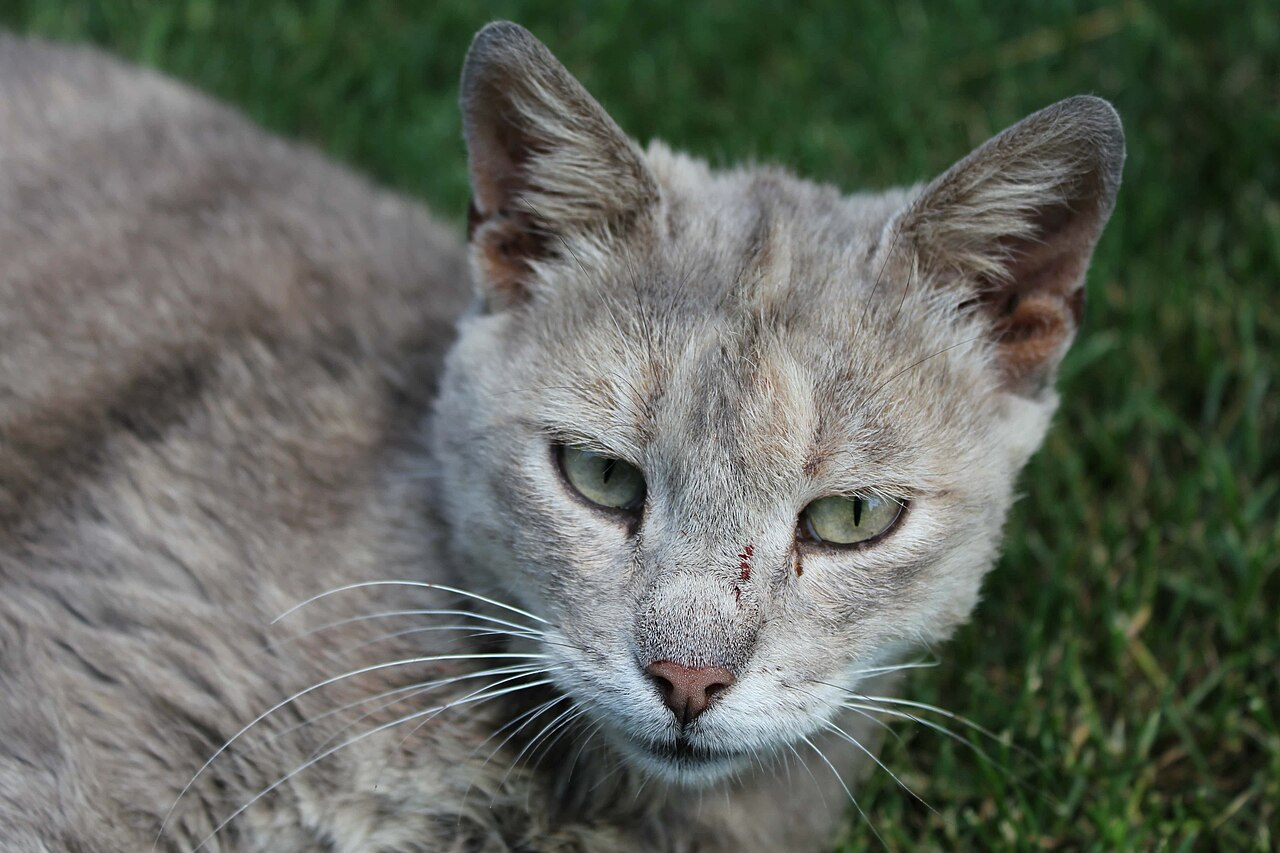
\includegraphics[width=0.7\textwidth]{Diagram/sample-cat.jpg}
    \caption{A single figure. Paths are relative to the graphics root set in \texttt{local\_paths.tex} (default: \texttt{Figures/}).}
    \label{fig:sample-cat}
\end{figure}

\lipsum[7]


\section{Aims and Objectives}
\label{sec:objectives}
\subsection{Research Questions}

\lipsum[8]

\subsection{Thesis Structure}

The remainder of this thesis is organised as follows. Chapter~\ref{ch:methodology} presents the governing equations and numerical scheme; Chapter~\ref{ch:results} reports verification results and draws conclusions. Supplementary derivations are collected in Appendix~\ref{app:derivations}.


\chapter{Methodology}
\label{ch:methodology}

\lipsum[2]

\section{Governing Equations}
\label{sec:governing-equations}
\subsection{Conservation Form}

% \nomenclature{symbol}{description} entries feed the List of Symbols
% (built by makeindex -- see .latexmkrc and .vscode/settings.json).
The governing \ac{PDE} for a conserved scalar $\phi$ is written in conservation form as
\begin{equation}
    \frac{\partial \phi}{\partial t} + \nabla \cdot \left( \bm{u}\,\phi \right) = \nabla \cdot \left( \Gamma \nabla \phi \right) + S_\phi,
    \label{eq:transport}
\end{equation}
\nomenclature{$\phi$}{Conserved scalar quantity}
\nomenclature{$\bm{u}$}{Velocity vector, \si{\metre\per\second}}
\nomenclature{$\Gamma$}{Diffusion coefficient, \si{\metre\squared\per\second}}
\nomenclature{$S_\phi$}{Volumetric source term}
\nomenclature{$t$}{Time, \si{\second}}
where $\bm{u}$ is the velocity, $\Gamma$ the diffusion coefficient and $S_\phi$ a source term. Equation~\eqref{eq:transport} reduces to the heat equation when $\bm{u} = 0$. \lipsum[9]


\section{Numerical Scheme}
\label{sec:numerical-scheme}
\subsection{Spatial Discretisation}

\lipsum[10]

\subsection{Time Integration}

After spatial discretisation the \ac{PDE} becomes a system of \ac{ODE}s in time. The explicit update is summarised in Algorithm~\ref{alg:explicit-euler}. \lipsum[11]

\begin{algorithm}[ht!]
\caption{Explicit Euler time stepping for Equation~\eqref{eq:transport}.}
\label{alg:explicit-euler}
\begin{algorithmic}[1]
\Require initial field $\phi^0$, time step $\Delta t$, number of steps $N$
\For{$n = 0, 1, \dots, N-1$}
    \State compute fluxes $F^n$ from $\phi^n$
    \State $\phi^{n+1} \gets \phi^n + \Delta t \, F^n$
\EndFor
\Ensure $\phi^N$
\end{algorithmic}
\end{algorithm}


\section{Implementation}
\label{sec:implementation}
\subsection{Code Structure}

\lipsum[12]

\subsection{Simulation Parameters}

The parameters used throughout Chapter~\ref{ch:results} are listed in Table~\ref{tab:sample-params}. \lipsum[13]

% House style: booktabs rules only, bold headers, \midrule-delimited groups.
\begin{table}[ht!]
\centering
\caption{Simulation parameters for the sample benchmark.}
\label{tab:sample-params}
\begin{tabular}{lll}
\toprule
\textbf{Parameter} & \textbf{Symbol} & \textbf{Value} \\
\midrule
\multicolumn{3}{c}{Fixed parameters (all configurations)} \\
\midrule
Spatial cells          & $N_x$        & $128$ \\
Domain length          & $L_x$        & \SI{1.0}{\metre} \\
Diffusion coefficient  & $\Gamma$     & \SI{1e-3}{\metre\squared\per\second} \\
\midrule
\multicolumn{3}{c}{Varied parameters} \\
\midrule
Time step              & $\Delta t$   & $10^{-4}$, $10^{-3}$, \SI{1e-2}{\second} \\
Velocity               & $u$          & $0$, $0.5$, \SI{1.0}{\metre\per\second} \\
\bottomrule
\end{tabular}
\end{table}


\chapter{Results and Conclusions}
\label{ch:results}

\lipsum[3]

\section{Verification Results}
\label{sec:verification}
\subsection{Convergence Study}

Figure~\ref{fig:sample-subfig} compares two configurations side by side. \lipsum[14]

% Sub-figure pair: each panel carries its own caption and label.
\begin{figure}[ht!]
    \centering
    \begin{subfigure}{0.48\textwidth}
        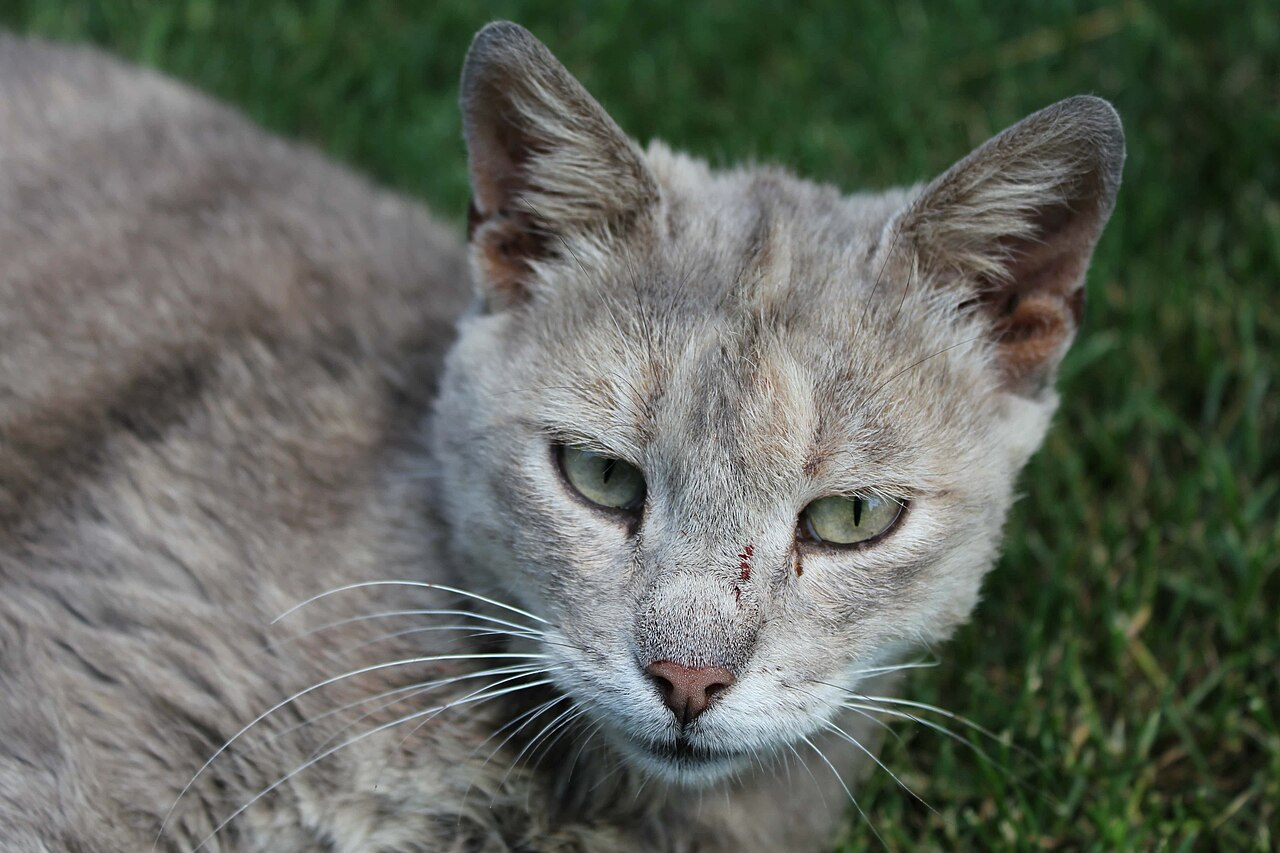
\includegraphics[width=\textwidth]{Diagram/sample-cat.jpg}
        \caption{Configuration A.}
        \label{fig:sample-subfig-a}
    \end{subfigure}
    \hfill
    \begin{subfigure}{0.48\textwidth}
        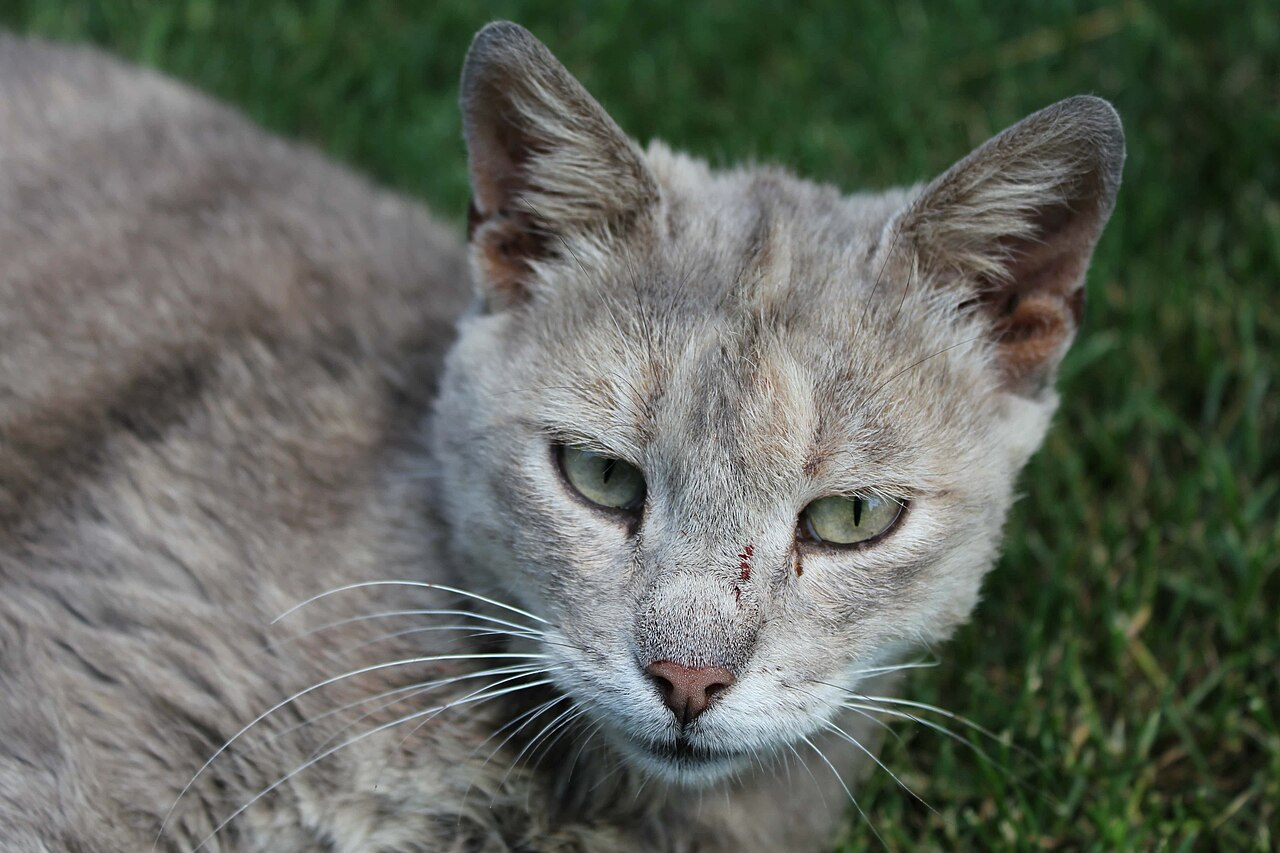
\includegraphics[width=\textwidth]{Diagram/sample-cat.jpg}
        \caption{Configuration B.}
        \label{fig:sample-subfig-b}
    \end{subfigure}
    \caption{Two sub-figures sharing one caption. \subref{fig:sample-subfig-a} and \subref{fig:sample-subfig-b} are referenced individually in the text.}
    \label{fig:sample-subfig}
\end{figure}

\lipsum[15]

\subsection{Discussion}

\lipsum[16]


\section{Conclusions and Future Work}
\label{sec:conclusions}
\subsection{Conclusions}

\lipsum[17]

\subsection{Future Work}

\lipsum[18]



% --- Bibliography ---
\clearpage
\addcontentsline{toc}{chapter}{Bibliography}
\bibliographystyle{ieeetr}
\bibliography{Thesis}

% --- Appendices ---
% Imperial's thesis submission guidance places appendices AFTER the bibliography.
\appendix

\chapter{Supplementary Derivations}
\label{app:derivations}
\section{Derivation of the Discrete Flux}
\label{app:flux}

Starting from Equation~\eqref{eq:transport}, \lipsum[19]



\end{document}
